\documentclass[11pt]{article}
\setlength{\topmargin}{-1.5cm}
\setlength{\textheight}{23cm}
\setlength{\oddsidemargin}{0mm}
\setlength{\evensidemargin}{0mm}
\setlength{\textwidth}{17cm}
\usepackage{graphicx, color}
\usepackage{amsmath, amssymb, amsthm}
\usepackage{enumerate}
\usepackage{hyperref}
\usepackage{verbatim}
\usepackage{placeins}

\newcommand{\problem}{\FloatBarrier \medskip \noindent \textbf}

\begin{document}
\noindent {\large  \textbf{Shawn Pan - CS 205 Homework 1, Spring 2017}} \medskip

\vspace{0.2in}

\problem{2 Analysis of Parallel Algorithms}

\problem{1}
The maximum degree of concurrency can be found by counting the number of leaf nodes.

\begin{enumerate}[a)]
\item 8
\item 7
\item 8
\end{enumerate}

\problem{2}
The critical path length is the longest path from the root to a leaf (depth of tree).

\begin{enumerate}[a)]
\item 8
\item 7
\item 8
\end{enumerate}

\problem{3}
\begin{enumerate}[a)]
\item 2 (1 processor for the critical path, and 1 for all the other nodes)
\item 2 (1 processor for the critical path, and 1 for all the other nodes)
\item 8 (last step requires 8 processors for maximum speedup)
\end{enumerate}

\problem{4}
The serial times can be found by counting the number of nodes, which are 15, 13, and 36 for the graphs.

For 2 processors:
\begin{enumerate}[a)]
\item 15/8 (2 processors is sufficient for max speedup)
\item 13/8 (2 processors is sufficient for max speedup)
\item 36/19 (only 1 processor can be used for the first job, and then the other 35 can be parallelized in 18 steps)
\end{enumerate}

For 5 processors:
\begin{enumerate}[a)]
\item 15/8 (2 processors is sufficient for max speedup)
\item 13/8 (2 processors is sufficient for max speedup)
\item 36/10 (5 steps for the 5 rows, and then the other 21 jobs can be parallelized in 5 steps)
\end{enumerate}

\newpage

\problem{3 Matrix Vector Multiplication}

\problem{Time-Optimal Solutions}
Time-optimal summation in $\log n$ steps was implemented and tested locally with $n=16$ and 8 processors.
A time-optimal matrix-vector multiplication is implemented by using the time-optimal summation for each row of the matrix-vector multiplication.
Because we would need $O(n^2)$ processors to actually see time-optimality, we did not actually observe a speedup.
In fact with only 8 processors, the parallel solution took over 300 times as long as the serial version.

\problem{Cost-Optimal Summation}
A parallel summation was implemented with Cython (with the prange function) and tested on Odyssey.
With 8 processors, we observed approximately 2.5 times speedup for larger problem sizes $n > 2^{20}$.
The speedup appears roughly constant as we scale to larger $n$.
This result corresponds to an efficiency of around 0.33.
For smaller problem sizes, the cost of managing parallization made the serial algorithm faster.

\begin{figure}[h!]
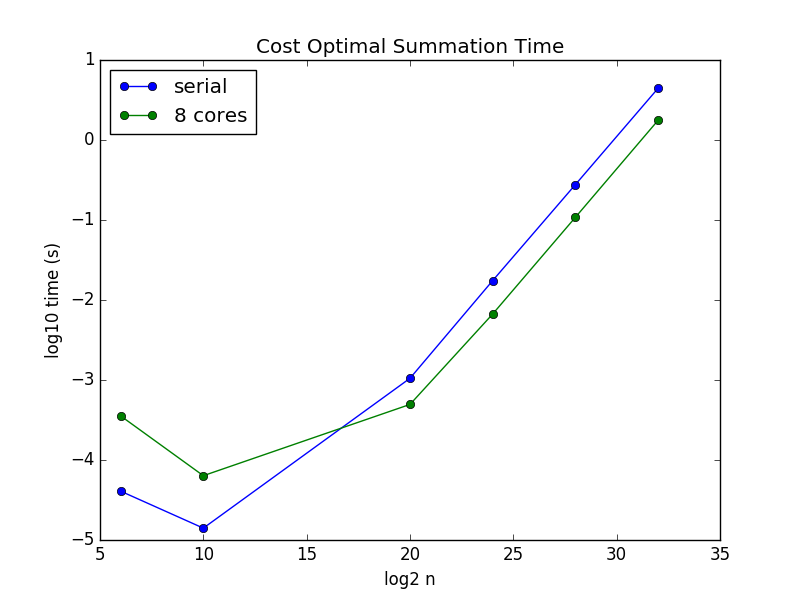
\includegraphics[width=5in]{problem3add.png}
\end{figure}

\begin{figure}[h!]
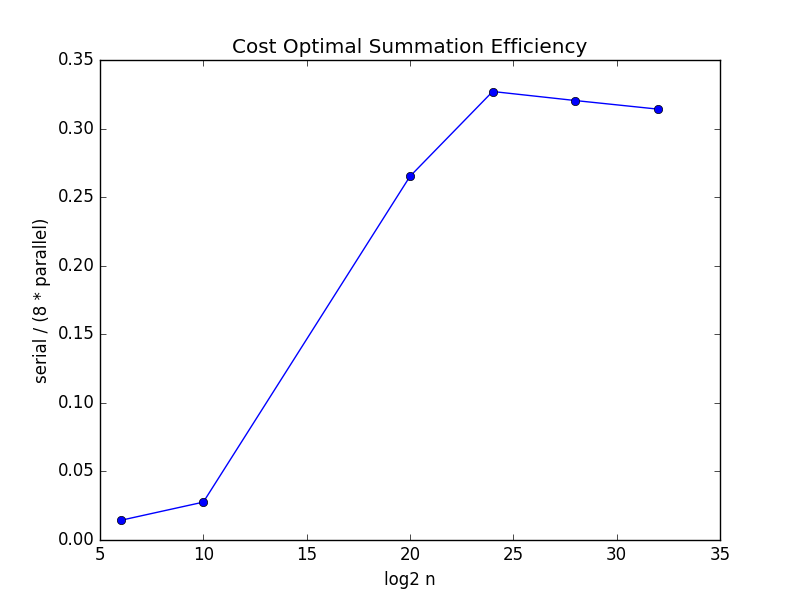
\includegraphics[width=5in]{problem3addeff.png}
\end{figure}

\problem{Cost-Optimal Matrix-Vector Multiplication}
A parallel matrix-vector multiplication was implemented with Cython (with the prange function) and tested on Odyssey.
With 8 processors, we observed approximately 4 times speedup for larger problem sizes $n > 2^{12}$.
The speedup appears roughly constant as we scale to larger $n$.
This result corresponds to an efficiency of around 0.5.
For smaller problem sizes, the cost of managing parallization made the serial algorithm faster.

Matrix-vector multiplication runs serially in $O(n^2)$.
To be cost-optimal, we want the parallel algorithm to run in $O(\frac{T_1}{p}) = O(\frac{n^2}{p})$

\begin{figure}[h!]
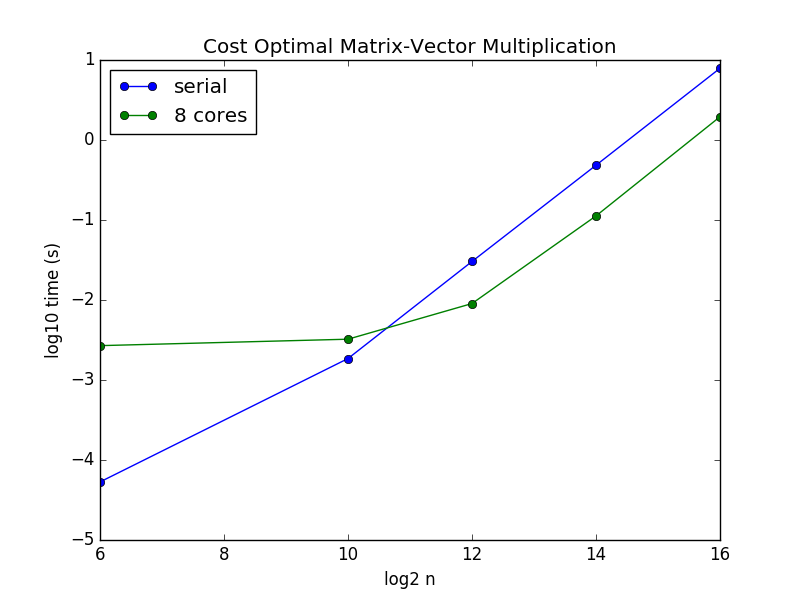
\includegraphics[width=5in]{problem3mv.png}
\end{figure}

\begin{figure}[h!]
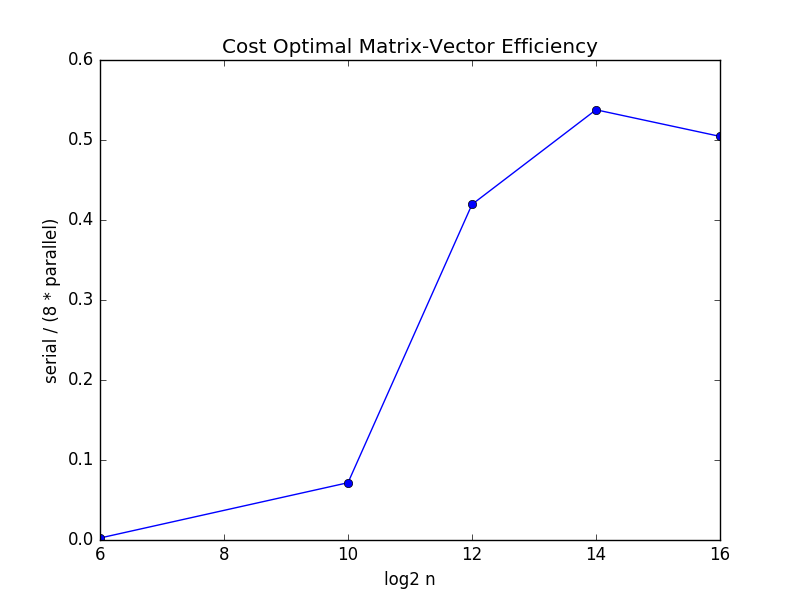
\includegraphics[width=5in]{problem3mveff.png}
\end{figure}



\problem{4 Matrix Matrix Multiplication}

We implemented and benchmarked the following matrix-multiplication algorithms.
We tested these algorithms for problem sizes $n=2^{6}$ to $n=2^{12}$ on an Odyssey compute node with 32 processors and 128 GB RAM.

\begin{enumerate}
\item BLAS dgemm (scipy implementation)
\item serial (3 nested loops)
\item parallel (3 nested loops, outermost loop parallelized with prange)
\item parallel + block (parallel with blocking for efficient memory caching)
\item parallel + strassen (parallel with Strassen's algorithm for reducing large problems to cache size)
\end{enumerate}

Our first attempt in making a fast algorithm is to simply parallelize the outermost loop.
Because all the calculations inside the outermost loop are independent, we expect the problem to be highly parallizable.
For larger problems sizes, we observed a 23 times speedup for $n = 2^{10}$ and a 21 times speedup for $n = 2^{12}$ over the serial version.
The ideal speedup expected would be 32 times, so we have an efficiency of around 0.7.
Interestingly, for $n= 2^8$ we get a 45 times speedup, which could due to a caching effect as described below or just measument error (results were on the order of milliseconds).

Our next attempt is to exploring blocking.
Because processors have a fast memory cache, we would like to reuse the data from the fast memory.
An Odyssey node has the following cache sizes, we pick a block size $b=256$ so that $3 \times 8 \textrm{bytes per double} \times b^2$ is less than the cache size.
With blocking, we observed a 120 times speedup for $n = 2^{10}$ and a 135 times speedup for $n = 2^{12}$ over the serial version.
\begin{verbatim}
Thread(s) per core:    2
Core(s) per socket:    8
Socket(s):             4
L1d cache:             16K
L1i cache:             64K
L2 cache:              2048K
L3 cache:              6144K
\end{verbatim}

Finally, we implemented Strassen's algorithm, which recusively divides the matrix multiplication problem.
Strassen's algorithm makes a tradeoff such that it only needs to do 7 half-sized $O(n^3)$ multiplication problems at the expense of many additional $O(n^2)$ addition steps.
By the master's theorem, this algorithm run asymptotically in $O(n^{\log_2 7}) \approx n^{2.8}$, which is better than $n^3$.
Emperically, we got the best performance by applying Strassen's algorithm recursively until $n = 64$ and then using our parallel implementation.
Note that this chunk size is smaller than the cache size.
The overhead of the added complexity is large, but for $n = 2^{12}$ we observed a 202 times speedup over the serial version.
For $n= 2^{12}$ and $n=2^14$ our Strassen implementation is better than our blocking implementation and almost as good as BLAS.
Thus, for large problem sizes the asymptotic complexity advantage becomes noticeable.

Overall, the scipy blas dgemm algorithm is very good, although our best parallel implementation with Strassen's algorithm comes very close.

\begin{figure}[h!]
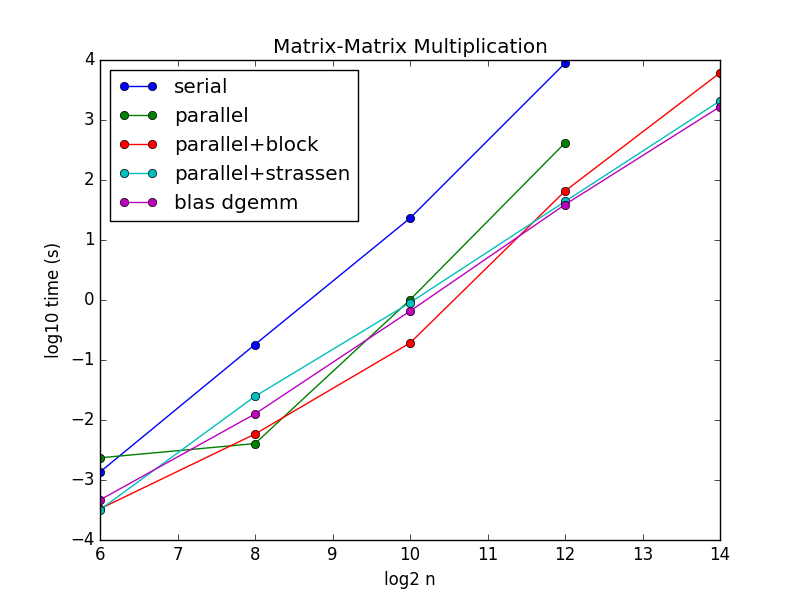
\includegraphics[width=5in]{problem4.png}
\end{figure}

\begin{figure}[h!]
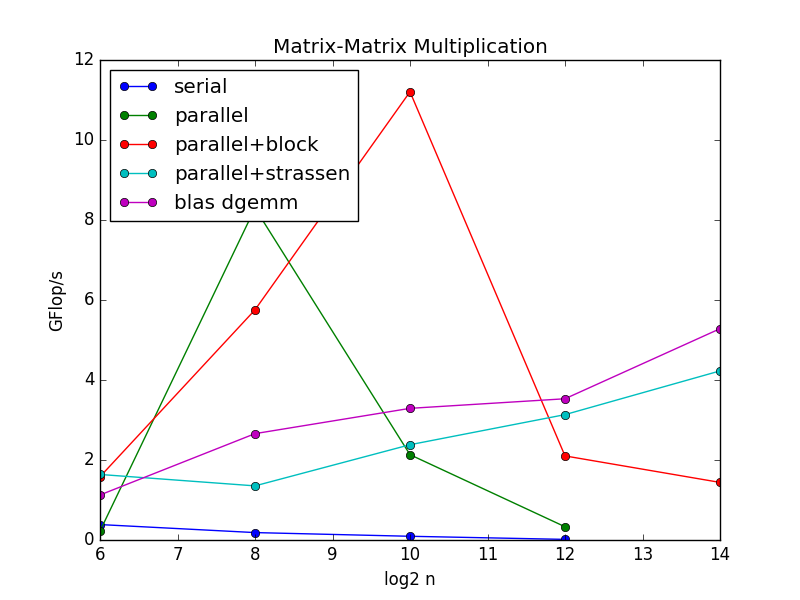
\includegraphics[width=5in]{problem4gflop.png}
\caption{We computed GFlop/s by assuming $2n^3$ floating point operations. Note that the Strassen results should be thought of as equivalent GFlop/s for comparisons rather than actual operations, because it only uses $O(n^{2.8})$ operations. The peak throughput is around 11 GFlop/s for problems small enough to remain in cache.}
\end{figure}


\end{document}


